\documentclass{lab}
\usepackage{amsmath}
\graphicspath{{pics/}}

\title {Лабораторная работа 3.2.5}
\author {Сидорчук Максим, Б01-304}
\date{\today}

\begin{document}
\maketitle

\section{Аннотация}
В данной работе проводится исследование вынужденных колебаний и процессов их установления под воздействием внешней ЭДС, которая гармонически меняется со временем; а также расчёт добротности контура несколькими способами: через исследование резонансных кривых, процессов установления и затухания колебаний; а также теоретически.
\section{Теоретические сведения}

Колебания в RLC-контуре представляют собой суперпозицию двух синусоид:
\begin{equation}
    I= B e^{-\gamma t} \sin (\omega t - \Theta)+ \frac{\mathcal{E}_0 \Omega}{L \rho_0} \sin (\Omega t - \psi),
    \label{law}
\end{equation}
При подключении контура к синусоидальной ЭДС собственные колебания с частотой $\omega$ со временем затухают. Однако при совпадении внешней частоты $ \Omega $ и собственной $ \omega $ возникает резонанс, при котором амплитуда вынужденных колебаний достигает максимального значения. Зависимость амплитуды установившихся колебаний от внешней частоты называется резонансной кривой.

Для достоверного исследования резонансной кривой необходимо, чтобы импеданс исследуемого участка цепи не зависел от импеданса источника питания даже на резонансе. С этой целью в работе используется параллельный колебательный контур
\begin{figure}
    \centering
    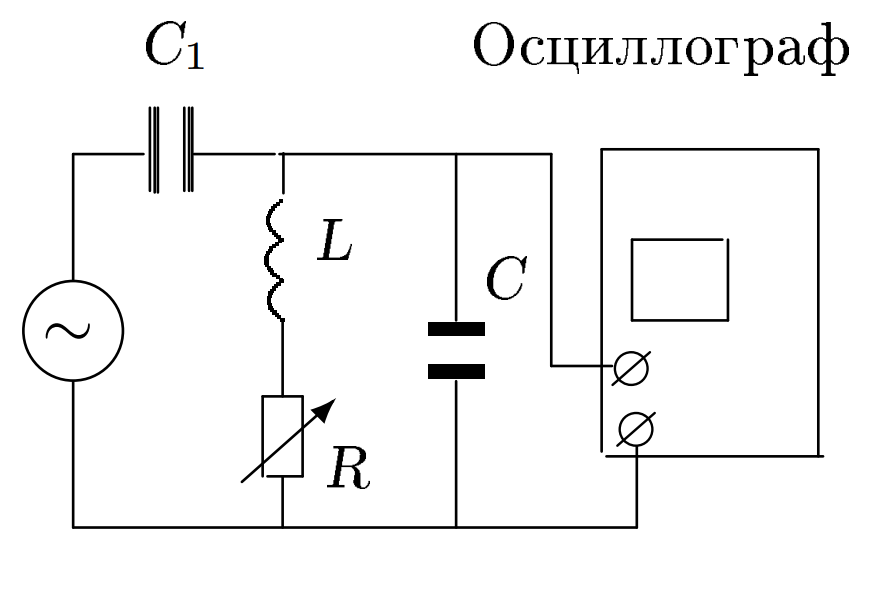
\includegraphics[width=0.8\textwidth]{Screenshot_1.png}
    \caption{Схема параллельного колебательного контура}
    \label{fig:scheme}
\end{figure}
Зависимость напряжения для конденсатора $ C \cdot U(\Omega) $ будет практически такой же, как в последовательном контуре при условии, что импедансы возбуждающей и измеряющей цепей существенно больше, чем импеданс исследуемой цепи. Таким образом,
\begin{equation}
    \frac{1}{\omega C_1}\gg \frac{L}{R C}, \; \; R_O \gg \frac{L}{R C},
\end{equation}
где $ R_O \simeq 1$ Ohm -- сопротивление на входе осциллографа.

По ширине резонансной кривой определяется добротность контура из формулы:
\begin{equation}
    Q = \frac{\omega_0}{2 \Delta \Omega} = \frac{\nu_0}{\Delta \nu},
    \label{eq:main}
\end{equation}
где $ \omega_0 = 2 \pi \nu_0 $ -- резонансная циклическая частота.

Добротность контура также можно определить по скорости возрастания амплитуды вынужденных колебаний, а также по скорости затухания свободных при резонансном значении частоты (что немаловажно). Обоими этими способами можно воспользоваться, если подавать колебания в контур цугами, то есть отрезками синусоиды в несколько периодов.

\subsection{Расчётные формулы}

\emph{Все формулы и расчёты приведены в системе СИ.}

Теоретическое определение резонансной частоты проводится по формуле:
\begin{equation}\label{nu}
    \nu_0 = \frac{1}{2 \pi \sqrt{L C}}
\end{equation}

Для определения добротности первым способом будем использовать формулу \ref{eq:main}, измеряя $ \Delta \Omega $ на уровне 0.7 от резонансной амплитуды.

Для определения вторым способом применим формулы:
\begin{equation}
    \Theta^\searrow = \frac{1}{n} \ln \frac{U_k}{U_{k+n}},
\end{equation}
\begin{equation}
    \Theta^\nearrow = \frac{1}{n} \ln \frac{U_0 - U_k}{U_0 - U_{k+n}},
\end{equation}
\begin{equation}
    Q = \frac{\pi}{\Theta}.
\end{equation}

Добротность также можно рассчитать теоретически через параметры контура по формуле:
\begin{equation}\label{teor}
    Q = \frac{1}{R } \sqrt{\frac{L}{C}}
\end{equation}

\section{Оборудование}
\begin{figure}[h!]
    \centering
    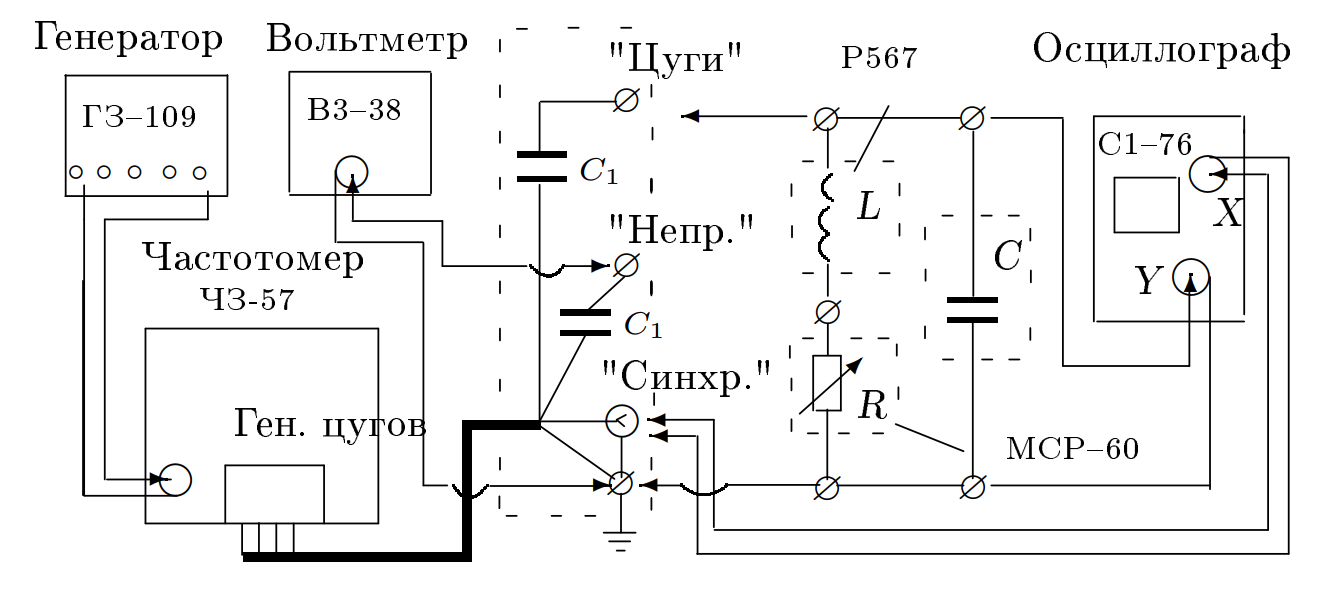
\includegraphics[width=1\linewidth]{Screenshot_2}
    \caption{Схема экспериментальной установки}
    \label{fig:set}
\end{figure}

\section{Результаты измерений и обработка данных}

\subsection {Нахождение критического сопротивления}

Для нахождения критическог сопротивления было произведено измерение зависимости логарифмического декремента затухания от сопротивления магазина:

\begin{table}[h!]
    \begin{center}
        \begin{tabular}{|c|c|c|c|c|c|c|c|}
            \hline
            $N$       & 1       & 2       & 3     & 4     & 5     & 6     & 7     \\ \hline
            $R$       & 370     & 740     & 1100  & 1480  & 1850  & 2200  & 2590  \\ \hline
            $\Theta$  & 0.357   & 0.630   & 0.953 & 1.272 & 1.615 & 2.036 & 2.391 \\ \hline
        \end{tabular}
    \end{center}
\end{table}

По теории, $R_{cr}^{thr} = 2 sqrt{L}{C} = 7313.5$ Ом.

Экспериментально было получено значение $R_{cr}^{real} = 7400$ Ом.

Построим график $\frac{1}{\Theta^2} = f (\frac{1}{R_\Sigma^2})$

\begin{figure}[h!]
\begin{center}
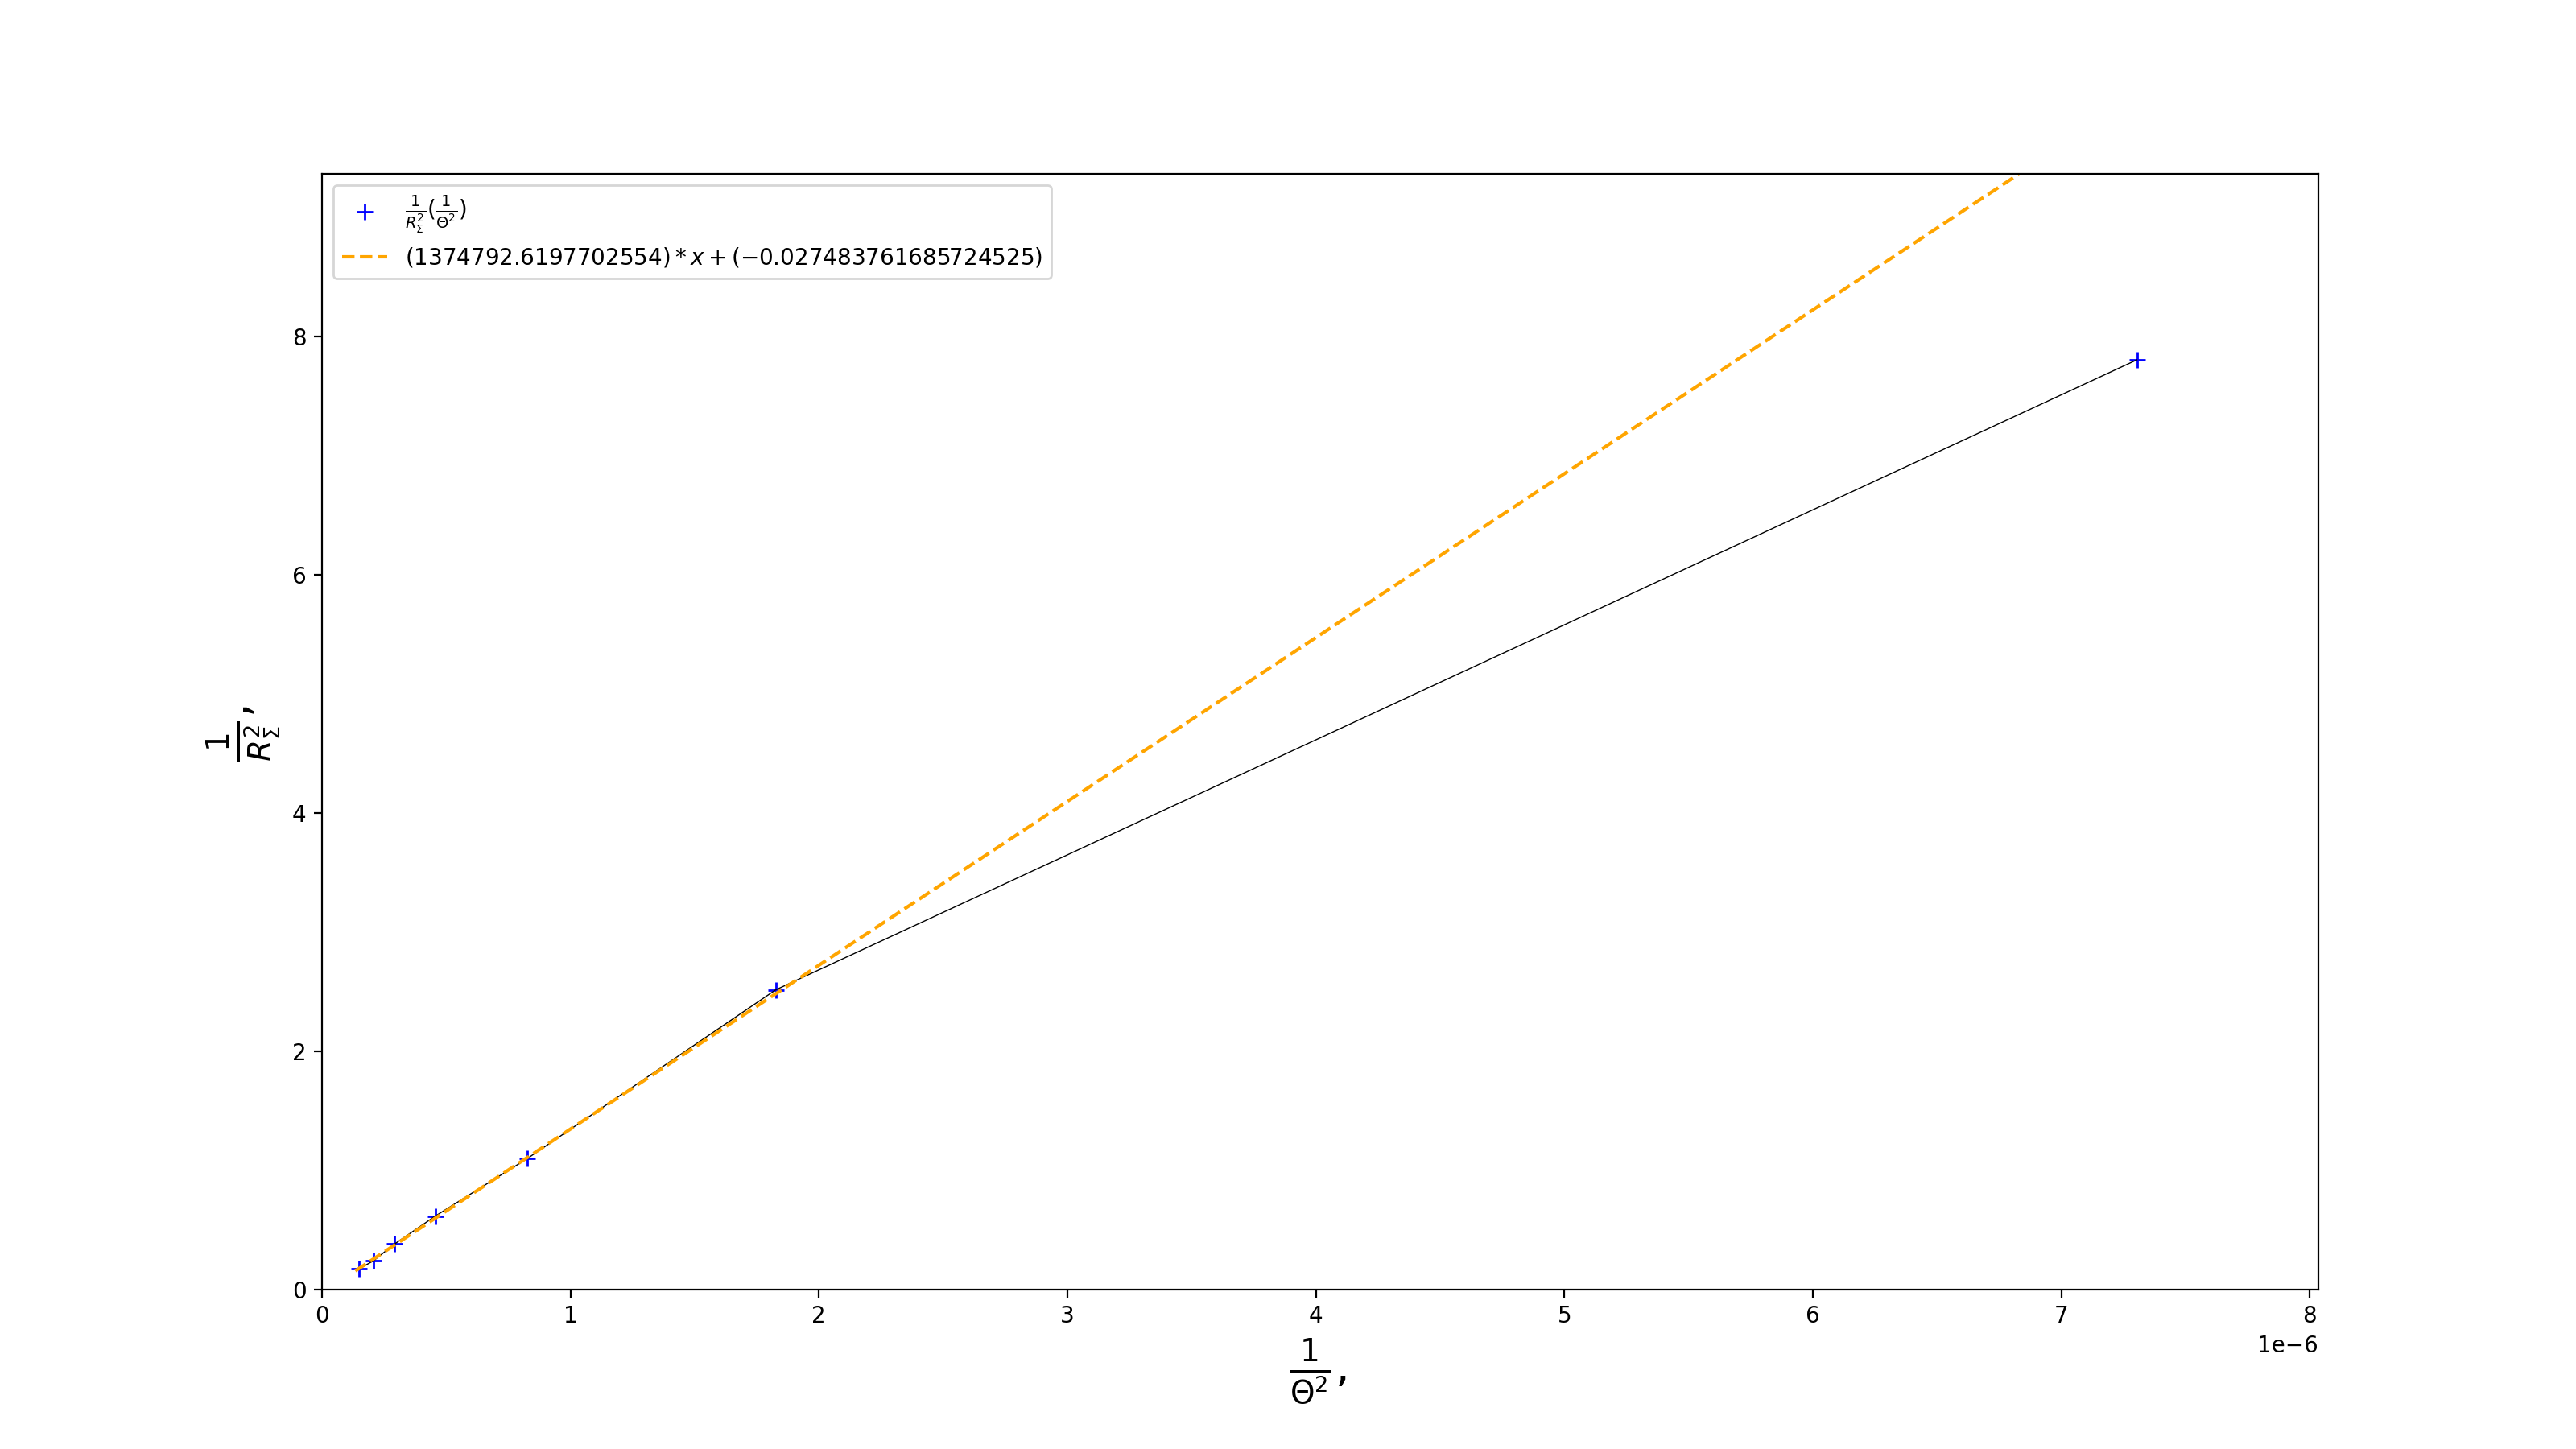
\includegraphics[width=1\textwidth]{graph1.png}
\end{center}
\end{figure}

Из наклона прямой на первых 6 точках определим критическое сопротивление.

$R_{cr}^{thr2} = 7599.29$ Ом

\subsection{Исследование резонансных кривых}

По формуле \ref{nu} рассчитаем теоретическую частоту резонанса:
\begin{equation}
    \nu_0\approx 1592 \; \text{Гц}
\end{equation}
\begin{equation}
    \nu_0^\text{эксп} \approx 1574 \; \text{Гц}.
\end{equation}
В таблице \ref{res} указаны резонансные значения напряжений

\begin{table}[]
    \centering
    \begin{tabular}{|l|l|l|}
        \hline
        \textbf{$R$, Ом} & \textbf{$\nu_0$, Гц} & \textbf{$U_0$, В} \\ \hline
        0                & 1574                 & 8.6               \\ \hline
        100              & 1574                 & 1.9               \\ \hline
    \end{tabular}
    \caption{Резонансные значения}
    \label{res}
\end{table}

Результаты исследования резонансных кривых отображены в таблице \ref{tabb}, по которым был построен график на рис. \ref{fig:graph} в безразмерных координатах.
\begin{table}[]
    \centering
    \begin{tabular}{|l|l|l|l|}
        \hline
        \multicolumn{2}{|l|}{\textbf{R=450 Ом}}         & \multicolumn{2}{l|}{\textbf{R=1250 Ом}}        \\ \hline
        \textbf{Частота, Гц} & \textbf{Напряжение, В} & \textbf{Частота, Гц} & \textbf{Напряжение, В} \\ \hline
        5700 & 4.1 & 5000 & 1.66 \\\hline
        5911 & 5.3 & 5157 & 1.82 \\\hline
        6122 & 7.0 & 5315 & 2.06 \\\hline
        6333 & 8.9 & 5473 & 2.3 \\\hline
        6544 & 9.7 & 5631 & 2.56 \\\hline
        6755 & 8.3 & 5789 & 2.94 \\\hline
        6966 & 6.9 & 5947 & 3.3 \\\hline
        7177 & 5.7 & 6105 & 3.46 \\\hline
        7388 & 4.8 & 6263 & 3.76 \\\hline
        7600 & 4.2 & 6421 & 3.86 \\\hline
        &     & 6578 & 3.98 \\\hline
        &     & 6736 & 3.94 \\\hline
        &     & 6894 & 3.86 \\\hline
        &     & 7052 & 3.72 \\\hline
        &     & 7210 & 3.62 \\\hline
        &     & 7368 & 3.38 \\\hline
        &     & 7526 & 3.2 \\\hline
        &     & 7684 & 3.1 \\\hline
        &     & 7842 & 2.94 \\\hline
        &     & 8000 & 2.86 \\\hline
    \end{tabular}
    \caption{Исходные данные для резонансных кривых}
    \label{tabb}
\end{table}
\begin{figure}[bth]
    \centering
    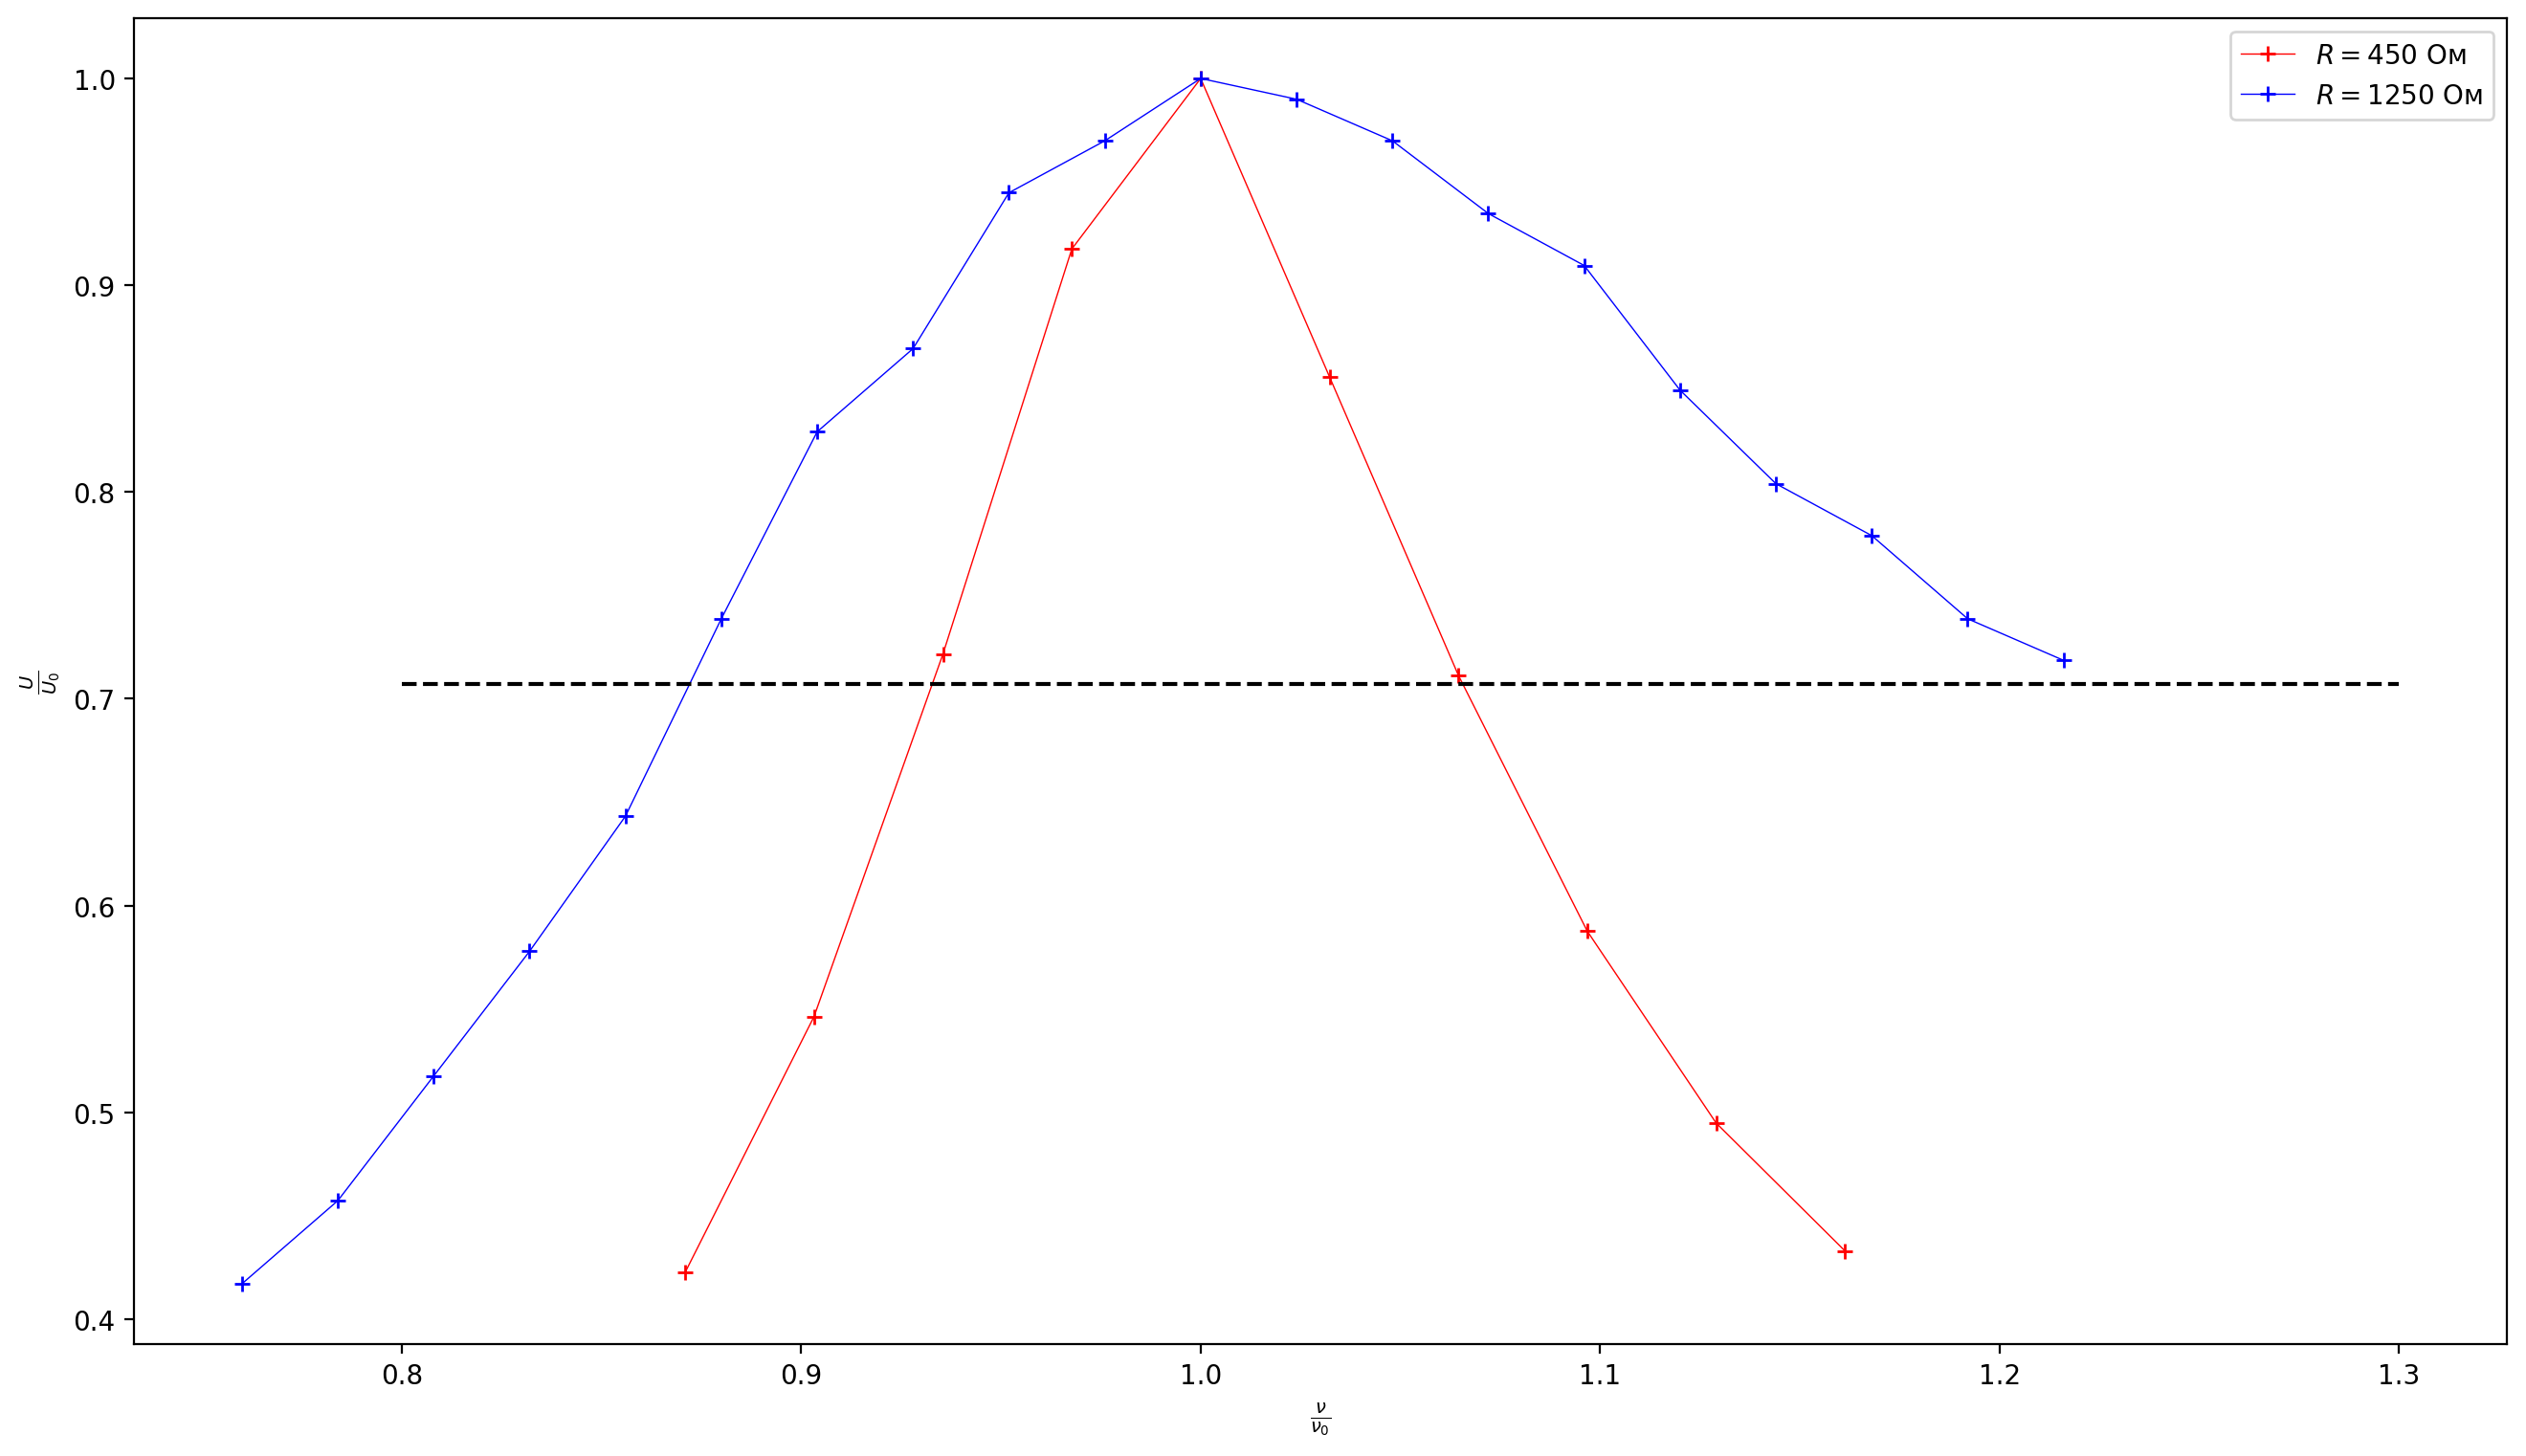
\includegraphics[width=1\linewidth]{G3}
    \caption{График резонансных кривых в безразмерных координатах $\frac{U}{U_0}(\frac{\nu}{\nu_0})$}
    \label{fig:graph}
\end{figure}
По нему на уровне $ U/U_0 = \frac{1}{\sqrt{2}}  $ определим ширину резонансной кривой и по формуле \eqref{eq:main} рассчитаем:
\begin{equation*}
    \Delta (\frac{\nu}{\nu_0})_{R=450} = 0.16 \pm 0.03,
\end{equation*}
\begin{equation*}
    \Delta (\frac{\nu}{\nu_0})_{R=1250} = 0.38 \pm 0.07 ,
\end{equation*}
\begin{equation}
    Q_{R=450} = \frac{1}{0.16} = 6.25,
\end{equation}
\begin{equation}
    Q_{R=1250} = \frac{1}{0.38} = 2.61,
\end{equation}

\subsection{Исследование установления и затухания колебаний}

Для каждого расчета построим таблицу.

\begin{table}[h!]
    \centering
    \begin{tabular}{|l|l|l|l|l|}
        \hline
        $\mathbf{U_k}$ & $\mathbf{U_{k+n}}$ & $\mathbf{n}$ & $\mathbf{\Theta}$ & $\mathbf{Q}$  \\ \hline
        3.4   & 5.4     & 1   & 0.42 & 8.38  \\ \hline
        5.4   & 6.8     & 1   & 0.49 & 8.20  \\ \hline
        6.9   & 8       & 1   & 0.59 & 6.58  \\ \hline
        7.9   & 8.6     & 1   & 0.53 & 6.83 \\ \hline
    \end{tabular}
    \caption{Расчёт добротности на установлении при $R=450$}
\end{table}

\begin{table}[h!]
    \centering
    \begin{tabular}{|l|l|l|l|l|}
        \hline
        $\mathbf{U_m}$ & $\mathbf{U_{m+n}}$ & $\mathbf{n}$ & $\mathbf{\Theta}$ & $\mathbf{Q}$ \\ \hline
        9.4 & 6.3 &  1           & 0.40                 & 7.85         \\ \hline
        6.3 & 4.2 &  1           & 0.41                 & 7.74         \\ \hline
        4.2 & 3.0 &  1           & 0.33                 & 9.33         \\ \hline
        3.0 & 2.0 & 1            & 0.41                 & 7.75         \\ \hline
    \end{tabular}
    \caption{Расчёт добротности на затухании при $R=450$}
\end{table}

\begin{table}[h!]
    \centering
    \begin{tabular}{|l|l|l|l|l|}
        \hline
        $\mathbf{U_k}$ & $\mathbf{U_k+n}$ & $\mathbf{n}$ & $\mathbf{\Theta}$ & $\mathbf{Q}$ \\ \hline
        1.2 & 2.84  & 0.76 & 4.13 & \\ \hline
        2.84 & 3.68 & 0.87 & 3.58 & \\ \hline
        3.8 & 4.08  & 0.87 & 3.58 & \\ \hline
    \end{tabular}
    \caption{Расчёт добротности на установлении при $R=1250$ Ом}
\end{table}

\begin{table}[h!]
    \centering
    \begin{tabular}{|l|l|l|l|l|}
        \hline
        $\mathbf{U_m}$ & $\mathbf{U_m+n}$ & $\mathbf{n}$ & $\mathbf{\Theta}$ & $\mathbf{Q}$ \\ \hline
        4.28 & 4.0  & 0.36 & 46.43  & \\ \hline
        4    & 1.6  & 0.86 & 3.42   & \\ \hline
        1.6  & 0.84 & 0.55 & 4.87   & \\ \hline
    \end{tabular}
    \caption{Расчёт добротности на затухании при $R=1250$ Ом}
\end{table}

Усредним эти значения:

\begin{equation}
    Q_{R=450} = 7.83 \pm 1.5
\end{equation}
\begin{equation}
    Q_{R=1250} = 3.97 \pm 1.5
\end{equation}

\subsection{Теоретический расчёт}

Определив параметры контура, занесём их в таблицу \ref{2}.

\begin{table}[h!]
    \centering
    \begin{tabular}{|l|l|l|}
        \hline
        $\mathbf{\nu}${\bf,  Гц} & $\mathbf{L}${\bf, мГн} & $\mathbf{R}${\bf, Ом} \\ \hline
        50                       & 100                    & 44.6                \\ \hline
        500                      & 99.953                 & 44.3                \\ \hline
        1500                     & 99.961                 & 45.9                \\ \hline
    \end{tabular}
    \caption{Параметры RLC-контура}
    \label{2}
\end{table}

На их основе рассчистаем $Q$:
\begin{equation}
    Q_{R=450} = 6.739 \pm 0.4
\end{equation}
\begin{equation}
    Q_{R=1250}= 2.574 \pm 0.3
\end{equation}
\end{document}
